\documentclass[a4paper,12pt,twocolumn]{article}
\usepackage{tabularx} % extra features for tabular environment
\usepackage{amsmath}  % improve math presentation
\usepackage{graphicx} % takes care of graphic including machinery
\usepackage[margin=1in,letterpaper]{geometry} % decreases margins
\usepackage{cite} % takes care of citations
\usepackage[final]{hyperref} % adds hyper links inside the generated pdf file
\usepackage{booktabs,caption, subcaption, multicol}
\usepackage{threeparttable}
\usepackage{graphicx} 
\usepackage{float}
\hypersetup{
	colorlinks=true,       % false: boxed links; true: colored links
	linkcolor=black,        % color of internal links
	citecolor=black,        % color of links to bibliography
	filecolor=magenta,     % color of file links
	urlcolor=black         
}

\begin{document}

\begin{titlepage}
	\begin{center}
		
		\thispagestyle{empty}
		
		\Huge{
			\textbf{UCD School Of Physics}
		}
		
		\vspace{1cm}	
		
		
\includegraphics[scale=0.08]{UCDLogo.png}
		
		\vspace{1cm}
		
		\large{
			\textbf{PHYC30170 Physics with Astronomy and Space Science Lab 1; \\
				Frequency Dependence of the Skin Depth in a Metal Cylinder \\
				\vspace{1cm}
				22/09/2022 \\
				\vspace{1cm}
				Daragh Hollman}
		} \\
		
	\end{center}
\end{titlepage}

\twocolumn[
\begin{@twocolumnfalse}
	\begin{abstract}
		The aim of this experiment was to investigate the frequency dependence of the skin effect in varying metal cylindrical conductors, and measure their conductivity. This was accomplished by measuring the induced voltage in a pick-up coil wrapped on each cylinder.
	\end{abstract}
\end{@twocolumnfalse}
]

\section{Introduction}
	In this experiment
	
\section{Theory}
	The skin effect

	Present key equations without deriving.
	
	Faraday's law of induction presents the voltage across the pick-up coil as a function of time [REFERENCE]:
	\begin{equation}
		\scriptsize
		V(t) = - i \omega N_2 \left( \int_{0}^{R} B(r) \cdot 2\pi r dr + \int_{R}^{R'} B_0 \cdot 2\pi r dr \right) e^{i\omega t}
	\end{equation}
	where the first integral represents flux within the sample and the second integral represents flux outside the sample. $N_2$ is the number of turns in the pick-up coil, $R$ the radius of the sample cylinder and $R'$ the mean radius of the pick-up coil.\\
	
	Following the derivations carried out in [REFERENCE] it can be shown that Faraday's Law reduces to the following equation for the pick-up voltage as a linear equation dependent on skin depth:
	
	\begin{equation}
		\frac{V}{\nu} = \frac{a}{2} + b\delta
		\label{eq:line}
	\end{equation}
	where $a = 2\pi^2 N_2 B_0 (R'^2-R^2)$, $b = 2\pi^2 N_2 B_0 R$ and skin depth, $\delta = (\pi \sigma \mu)^{-1/2}$.
	
\section{Methodology}
	
	\begin{figure}
		\centering
		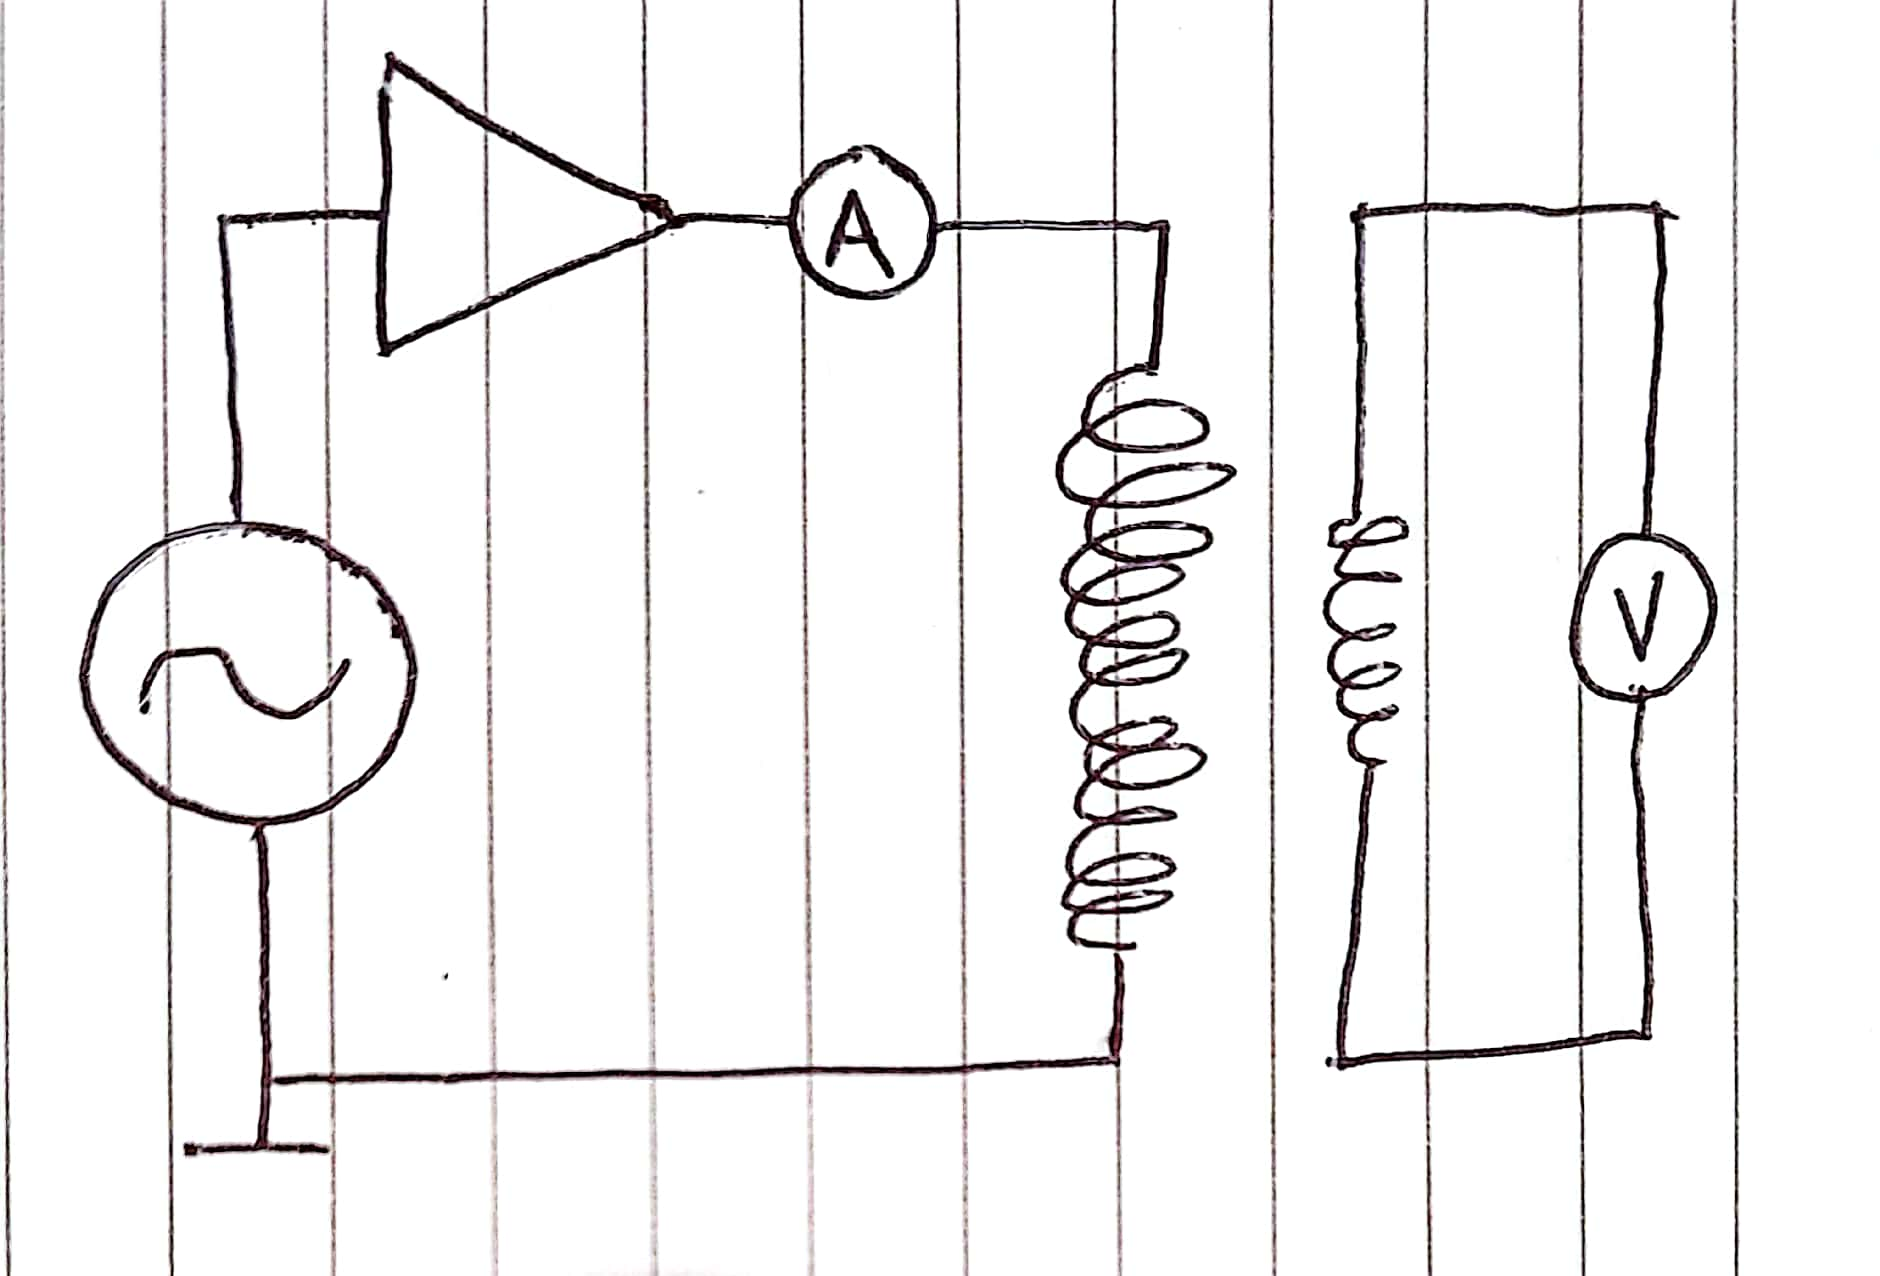
\includegraphics[scale=0.1]{SDcircuit.jpg}
		\captionsetup{font=scriptsize}
		\caption{Circuit diagram of the skin depth apparatus}
		\label{fig:circuit}
	\end{figure}

	\begin{figure}
		\centering
		\includegraphics[scale=0.045]{SDPhoto.jpg}
		\captionsetup{font=scriptsize}
		\caption{Photo of the skin depth apparatus, the metal cylinders were held inside the primary coil and  }
		\label{fig:photo}
	\end{figure}

	The apparatus was setup as shown in figures \ref{fig:circuit} and \ref{fig:photo}. The induction field was created by a solenoid of length $L_1 = (389 \pm 0.5) \,\text{mm}$ which contained $N_1 = (856 \pm 78)$ turns of an insulated copper wire wound on a hollow tube - which the metal cylinders were inserted into. The signal to this solenoid was created by an AC signal generator and amplified. The rms current was kept constant at $I = (19 \pm 0.1)\,\text{mA}$; Which was adjusted to adjust for each frequency due to the change in reactance. Although the accuracy of the ammeter used was higher, a larger uncertainty was used in practice to account for the very high sensitivity of adjusting the amplitude of the signal generator's output.\\
	
	Four cylinders were used, all of the same dimensions: Copper, aluminum, brass and steel. Each cylinder was wrapped at the middle with a pick-up coil, of the same insulated copper wire as the solenoid, containing $(100 \pm 10)$ turns. The tail ends of this coil were routed down the length and outside of the solenoid to where they could be connected to a voltmeter to take measurements. Voltages were measured from this pick-up coil for 30 frequencies between $6.5 \,\text{kHz}$ and $62.5 \,\text{kHz}$. This range was determined from the results of the same experiment carried out by H.D. Wiederick and N. Gauthier [REFERENCE]. These data were recorded and the voltage divided by the frequency ($V \nu^{-1}$) was plotted against the inverse of the square root of the frequency ($\nu ^{-1/2}$). This was repeated for all four cylinders.
	
\section{Results and Analysis}
	
	The voltage divided by the frequency ($V \nu^{-1}$) was plotted against the inverse of the square root of the frequency ($\nu ^{-1/2}$) for each cylinder in figures \ref{fig:copperGraph}, \ref{fig:aluminiumGraph}, \ref{fig:brassGraph} and \ref{fig:steelGraph}. Scatter plots were used to display the data and a linear least squares fit was used to calculate the slope of the linear portion of the data. At higher frequencies the data deviates significantly from the expected linear result and is hence excluded from the fit calculation. This is likely due to an unaccounted for increase in the emf induced in the pick-up coil by the rod due to charged particles becoming more concentrated at the surface of the material as the skin depth decreases. This however is primarily speculation, further experiments would need to be carried out to yield a conclusive reason.\\
	
	From these slopes, the conductivity of each material was calculated by comparing expression \ref{eq:line} with the linear fit to solve for the conductivity.\\
	
	\begin{equation}
		
	\end{equation}
	
	It could be inferred from the results that the steel was a carbon steel based on the conductivity calculated using its permeability.
	
	Discuss relative mu with respect to ferrous metals.
	
	Discuss error analysis
	
	Due to having higher voltages, the relative error on the brass and particularly the steel graph was reduced.
	
	\begin{figure*}
		\centering
		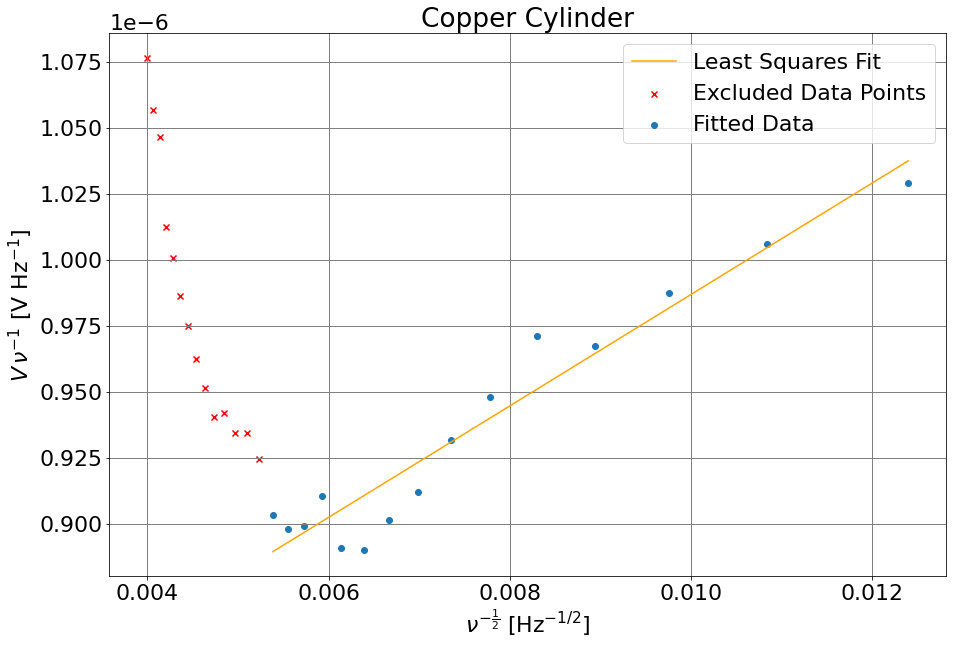
\includegraphics[scale=0.4]{copperGraph.png}
		\captionsetup{font=scriptsize}
		\caption{Copper Graph}
		\label{fig:copperGraph}
	\end{figure*}
	\begin{figure*}
		\centering
		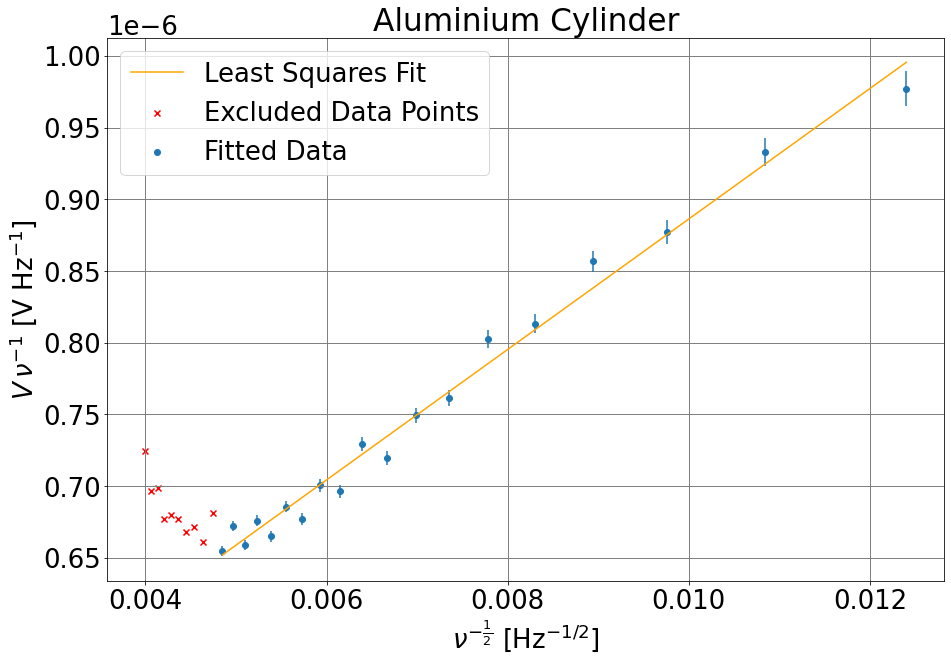
\includegraphics[scale=0.4]{aluminiumGraph.png}
		\captionsetup{font=scriptsize}
		\caption{Aluminium Graph}
		\label{fig:aluminiumGraph}
	\end{figure*}
	\begin{figure*}
		\centering
		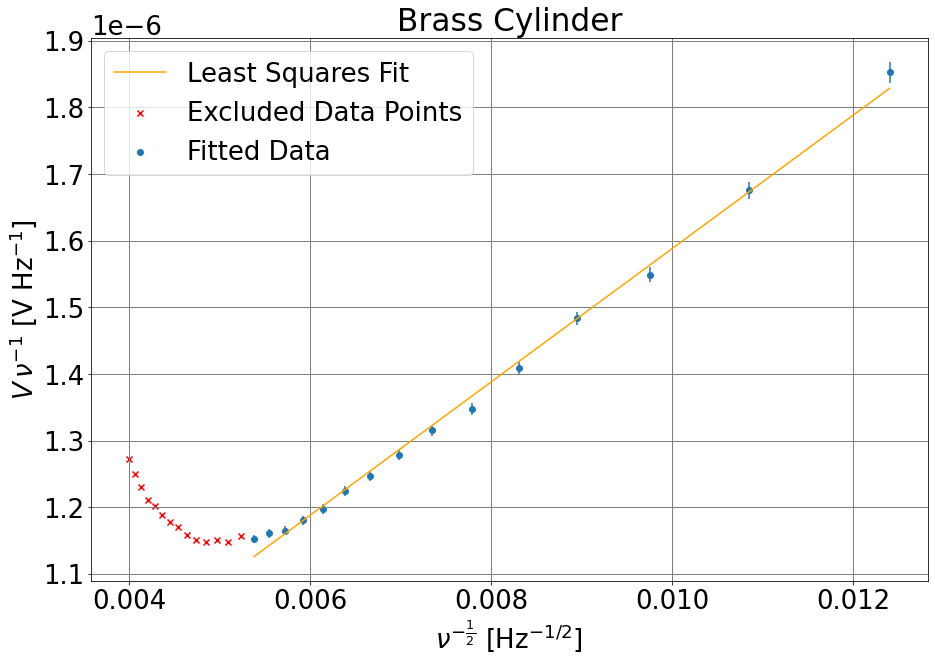
\includegraphics[scale=0.4]{brassGraph.png}
		\captionsetup{font=scriptsize}
		\caption{Brass Graph}
		\label{fig:brassGraph}
	\end{figure*}
	\begin{figure*}
		\centering
		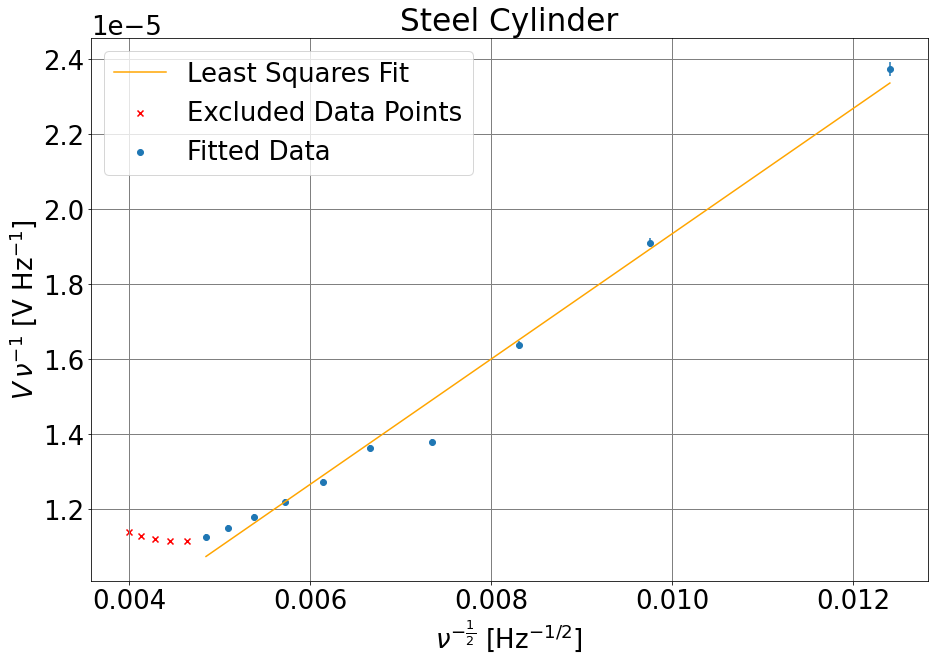
\includegraphics[scale=0.4]{steelGraph.png}
		\captionsetup{font=scriptsize}
		\caption{Steel Graph}
		\label{fig:steelGraph}
	\end{figure*}
	

\section{Conclusion}
	

\newpage
\begin{thebibliography}{}
	
	
\end{thebibliography}

	

\newpage

\section*{Appendices}
	
	
\end{document}
